%!TEX program = pdflatex
\documentclass[11pt,en]{elegantpaper}

\title{The Report for Programming Assignments in Chapter Four}
\author{Wenchong Huang}

\date{\today}

% cmd for this doc
\usepackage{array}
\usepackage{float}
\usepackage{pgfplots}
\usepackage{tikz}
\usepackage{graphicx}
\usepackage{subfigure}
\newcommand{\ccr}[1]{\makecell{{\color{#1}\rule{1cm}{1cm}}}}

\begin{document}

\maketitle


\section{How to Test}

Enter the folder \verb|Programming-Chapter4/src| with terminal, \verb |make| here, you will see some executable files whose names are corresponding assignments. Run them directly and you will see the results.

To get the figures in this report, run \verb|drawA.m| and \verb|drawB.m| with \textbf{matlab}.

\section{Results}

\subsection{Assignment A}

Please see the numerical result in \verb|Programming-Chapter4/src/A.txt|. We plot it here.

\begin{figure}[H]
    \centering
    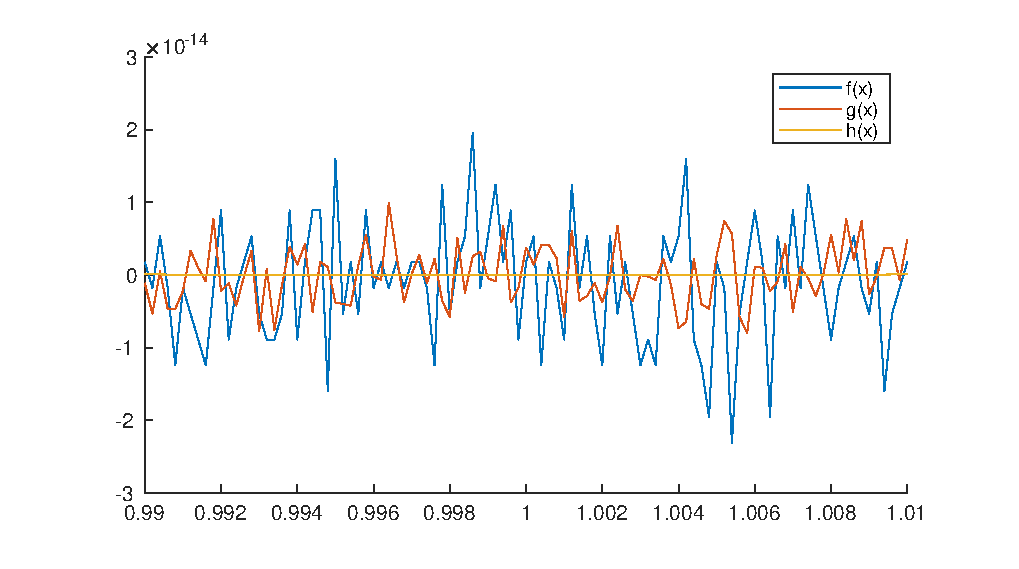
\includegraphics[width=0.8\textwidth]{figure/A.eps}
\end{figure}

We could see that $f(x)$ and $g(x)$ have strong oscillation. And $h(x)$ is the most accurate, $f(x)$ is the least accurate.

The reason is that we did lots of additions and subtractions of numbers which are very close in $f(x)$ and $g(x)$. And that caused catastrophic cancellations. However $h(x)$ only did subtraction once when calculate $x-1$. So $h(x)$ is much more accurate.

\subsection{Assignment B}

We consider the normalized FPN system $\mathbb{F}$ with $\beta=2,p=3,L=-1,U=1$.

\begin{enumerate}[(i)]
    \item $\text{UFL}(\mathbb{F})=0.5,\;\text{OFL}(\mathbb{F})=3.75$.
    \item The numbers in $\mathbb{F}$ are listed here.
    \begin{lstlisting}
        -3.5 -3 -2.5 -2 -1.75 -1.5 -1.25 -1 -0.875 -0.75 -0.625 -0.5 
        0 0.5 0.625 0.75 0.875 1 1.25 1.5 1.75 2 2.5 3 3.5
    \end{lstlisting}
    There are $33$ numbers, which supported the corollary on the cardinality.
    \item See the numbers in $\mathbb{F}$ in the following figure.
    \begin{figure}[H]
        \centering
        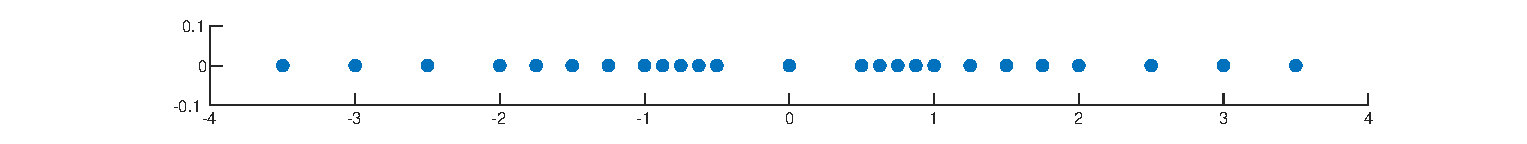
\includegraphics[width=\textwidth]{figure/FPN.eps}
    \end{figure}
    \item The subnormal numbers of $\mathbb{F}$ are listed here.
    \begin{lstlisting}
        -0.375 -0.25 -0.125 0 0.125 0.25 0.375
    \end{lstlisting}
    \item See the numbers of extended $\mathbb{F}$ in the following figure, where blue points are normal numbers and red points are subnormal numbers.
    \begin{figure}[H]
        \centering
        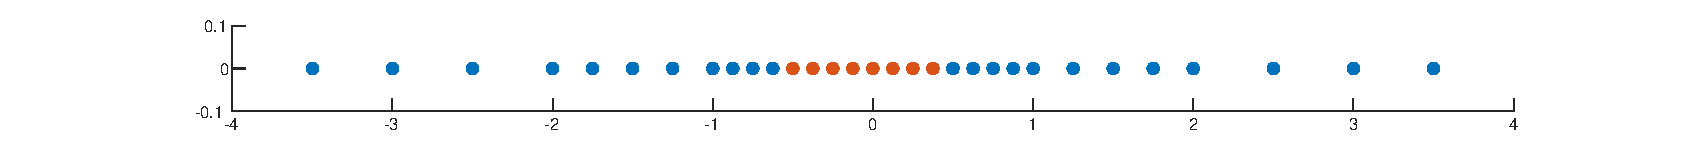
\includegraphics[width=\textwidth]{figure/FPNext.eps}
    \end{figure}
\end{enumerate}

\end{document}
